\label{section:outputs}
\setcounter{footnote}{0}
\section{Outputs}

For each alignment file \prog{rnafile.sto}, \rscape\, produces the
following output files:

\begin{sreitems}{\emprog{rnafile.sorted.out}}
\item[\emprog{rnafile.out}] Tabular output with the significant pairs,
  with their score and E-value.
%
\item[\emprog{rnafile.sorted.out}] Tabular output sorted from highest to
  lowest E-value.
%
\item[\emprog{rnafile.roc}] Tabular output that provides statistics for 
each score value.
%
\item[\emprog{rnafile.sum}] Tabular output with a line summary statistics
  per alignment in the file.
%
\end{sreitems}

\subsection{Tabular output per input file}

The distribution includes examples of output files. If you
run \rscape, the outputs will go into your current working directory
(not necessarily tutorials/).

The output file \emprog{tutorial/updated\_Arisong.out} looks like this:

\begin{sreoutput}
# MSA updated_Arisong_1 nseq 69 (95) alen 65 (150) avgid 65.16 (64.97) nbpairs 20 (20)
# Method Target_E-val cov_at_target_E-val [cov_min,conv_max] [FP | TP True Found | Sen PPV F] 
# GTp    0.05         41.31               [-9.74,89.08]     [2 | 9 20 11 | 45.00 81.82 58.06] 
#       left_pos       right_pos        score   E-value
#------------------------------------------------------------
                93             104      43.65   6.01567e-06
*               94             110      43.17   4.29923e-05
*               96             108      65.95   0
*               98             106      89.08   0
...
\end{sreoutput}
The output file is a tabular list of significant pairs sorted by sequence positions:

\begin{sreitems}{\prog{Second and third columns}}
 \item[\prog{First column}] indicates whether the significant pair is
   part of the given structure (*), or not.  If the pair is not in the
   structure, we distinguish whether the pair is compatible with the
   given structure ($\sim$) or not (blank).

 \item[\prog{Second and third columns}] are the two positions of the
   pair, $i\leq j$ respectively. Positions are relative to the input
   alignment.

 \item[\prog{Fourth column}] is the covariation score.

 \item[\prog{Fifth column}] is the E-value. Significant positions
   have E-values $<< 1$.
 \end{sreitems}
 The output file also includes two comment lines per alignment in the
 file:

 \begin{sreitems}{\prog{Second comment line}} \item[\prog{First
 comment line}]describes properties of the alignment: number of
 sequence (nseq), alignment length (alen), average percentage identity
 (avgid), and number of base pairs (nbpairs).  Values in parentheses
 correspond to the alignment as given. Values not in parentheses
 correspond to the analyzed alignment after the filters (for redundant
 sequences and gapped columns) have been applied.

 \item[\prog{Second comment line}]describes properties of the
   \rscape\ search: the covariation method (GTp), the E-value threshold
   (0.05), the score at that E-value (41.3), the range of scores for all
   pairs in the alignments (from -9.7 to 89.1), the number of covarying
   non base pairs (2), the number of covarying base pairs (9), the
   number of base pairs (20), and the total number of covarying pairs
   (11). Lastly we provide the sensitivity (SEN=45.0=9/20), positive
   predictive value (PPV=81.8=9/11), and F-measure (F=58.1 = 2 * SEN *
   PPV / (SEN+PPV)).
 \end{sreitems}


\subsection{Other tabular outputs}

 \rscape\ produces two more tabular outputs per input file that are
 more relevant for benchmarking purposes, those are:\\

 File \emprog{tutorial/updated\_Arisong.sum} looks like:

\user{more tutorial/updated\_Arisong.sum}
 \begin{sreoutput}
 #target_E-val   MSA                     nseq    alen    avgid    method  TP      True    Found   SEN     PPV
 0.050000        updated_Arisong_1       69      65      65.16    GTp      9        20       11   45.00   81.82 
 \end{sreoutput}
 This file produces a one line output per alignment in the file.
 \begin{sreitems}{\prog{Second column}}
 \item[\prog{Column 1}] Target E-value.
 \item[\prog{Column 2}] Alignment name.
 \item[\prog{Column 3}] Number of sequence in the analyzed alignment.
 \item[\prog{Column 4}] Number of columns analyzed.
 \item[\prog{Column 5}] Average percentage identity in the analyzed alignment.
 \item[\prog{Column 6}] Covariation statistic.
 \item[\prog{Column 7}] Number of significant base pairs, TP  (true positives).
 \item[\prog{Column 8}] Number of base pairs, T (True).
 \item[\prog{Column 9}] Number of significant pairs, F (Found).
 \item[\prog{Column 10}] Sensitivity = TP/T.
 \item[\prog{Column 11}] Positive predictive value = TP/F.

 \end{sreitems}

File \emprog{tutorial/updated\_Arisong.roc} looks like:

\user{more tutorial/updated\_Arisong.roc}
\begin{sreoutput}
 # MSA nseq 69 alen 65 avgid 65.163163 nbpairs 20 (20)
# Method: GTp
#cov_score  FP  TP  Found  True  Negatives   Sen   PPV     F       E-value
89.04630    0   1       1    20       2060   5.00  100.00  9.52    0
88.79103    0   1       1    20       2060   5.00  100.00  9.52    0
88.53575    0   1       1    20       2060   5.00  100.00  9.52    0
...
\end{sreoutput}

This file produces a tabular output for each alignment as a function
of the covariation score, for plotting ROC curves. The values in the
file are described by the comment line. Notice that the number of
Trues (column 5) and Negatives (column 6) are fixed for a given
secondary structure and do not change.

\subsection{Outputs per alignment}

A Stockholm alignment file can include several different multiple
sequence alignments (MSAs).  \rscape\ produces the following output
files, one for each individual alignment in the input Stockholm file:

\subsubsection{Alignment with consensus secondary structure}
If the given alignment  has a consensus secondary structure
(\prog{\#=GF SS\_cons} markup), the following files are produced

\begin{sreitems}{\emprog{rnafile\_msaname.R2R.sto.\{pdf,svg\}}}
\item[\emprog{rnafile\_msaname.R2R.sto}] Stockholm file annotated by a
  modified version of the R2R program. This file includes the
  information necessary to draw the consensus structure, and to
  annotate the significantly covarying base pairs.
%
\item[\emprog{rnafile\_msaname.R2R.sto.\{pdf,svg\}}] Drawing of the
  \rscape-annotated consensus secondary structure.
%
\item[\emprog{rnafile\_msaname.cdf}] A two column file with the 
cumulative distribution functions (cfg) for the covariation scores.
%
\item[\emprog{rnafile\_msaname.cdf.ps}] Plot of the score's cdf. Drawing this
file requires that program \emprog{gnuplot} is installed somewhere in the
\prog{\$\{PATH\}}, or that the environmental variable GNUPLOT 
pointing to a gnuplot executable is defined.
%
\item[\emprog{rnafile\_msaname.dplot.\{ps,svg\}}] Dot plot of the consensus
  secondary structure annotated according to covariation. Drawing of this
file requires that program \emprog{gnuplot} is installed somewhere in the
\prog{\$\{PATH\}}, or that the environmental variable GNUPLOT 
pointing to a gnuplot executable is defined.
%
\end{sreitems}
For each alignment, \emprog{msaname} is given
by \prog{<ACC>\_<ID>}, the combination of the accession \prog{\#=GF
AC <ACC>} and name \prog{\#=GF ID <ID>} in the Stockholm-format markups (or
one of two if the other in not defined).  If none of those fields are
defined, \emprog{msaname} is a number describing the order in the
file of the given alignment.

\subsubsection{Alignment without consensus secondary structure}
Alternatively, if the alignment does not have a consensus secondary
structure (or if it does and the option \prog{\rscape\ --cyk} is
used) \rscape\, produces the following files describing the
maximal-covariation optimal secondary structure:

\begin{sreitems}{\emprog{rnafile\_msaname.cyk.R2R.sto.\{pdf,svg\}}}
\item[\emprog{rnafile\_msaname.cyk.R2R.sto}]
%
\item[\emprog{rnafile\_msaname.cyk.R2R.sto.\{pdf,svg\}}]
%
\item[\emprog{rnafile\_msaname.cyk.cdf}]
%
\item[\emprog{rnafile\_msaname.cyk.cdf.\{ps.svg\}}]
%
\item[\emprog{rnafile\_msaname.cyk.dplot.\{ps,svg\}}]
%
\end{sreitems}
These files are formatted identically to those for describing the given
consensus structure.


\subsubsection{Details about outputs per alignment}
 Two files are produced per alignment in the input file: \\

 File \emprog{tutorial/updated\_Arisong\_1.R2R.sto} is a Stockholm
 formatted alignment that includes the input alignment annotated with
 the consensus structure. This Stockholm file also includes the
 additional annotation required to use the drawing program R2R.

 It is possible that the resulting drawing will show parts of the
 secondary structure occluded from each other (especially for long
 RNAs).  Using this file, one can customize a different drawing of the
 structure using the R2R documentation, provided in
 \prog{lib/R2R/R2R-manual.pdf}.\\

 File \emprog{tutorial/updated\_Arisong\_1.cdf} looks like this:

\user{more tutorial/updated\_Arisong.cdf}
 \begin{sreoutput}
 89.046301       0.000480769
 68.879658       0.000961538
 65.816370       0.00144231
 56.115959       0.00192308
 ...
 &
 41.054795       9.61538e-06
 40.799521       3.84615e-05
 40.288973       6.73077e-05
 ...
 &
 49.478836       2.13504e-20
 49.223562       4.27009e-20
 48.968288       1.06752e-19
 ...
 &
 \end{sreoutput}
 The first column is a covariation score (x). The second column is the
 survival function $P(X > x)$, that is the frequency of pairs having
 score larger than x. The file includes three cdfs separated by a
 ``\&'' line. The three cdf correspond to:

 \begin{sreitems}{\prog{Second cdf}}
 \item[\prog{First cdf}] the given alignment, all possible pairs.
 \item[\prog{Second cdf}] the aggregation of all null alignments, all possible pairs.
 \item[\prog{Third cdf}] the expected null cdf according to the tail Gamma fit.
 \end{sreitems}


\clearpage
\subsubsection{Graphical outputs per alignment}
 Three plots are produced per alignment in the input file: 

 \begin{figure}[h]
   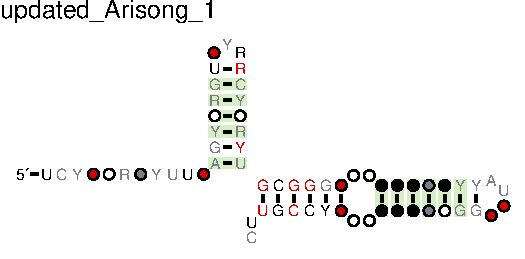
\includegraphics[scale=1.5]{Arisong_R2R.pdf} 
 \caption{\small\textbf{\emprog{tutorial/updated\_Arisong\_1.R2R.sto.\{pdf,svg\}}:
     annotated consensus secondary structure.} Base pairs with
   covariation scores equal or below the target E-value (0.05 as
   default) are depicted in green. By default only positions in the
   alignment with more than 50\% occupancy are depicted (unless they form
   a base pair). Option \prog{--r2rall} forces the depiction of all
   positions in the alignment.  }
 \label{fig:r2r}
 \end{figure}

 \begin{figure}[h]
   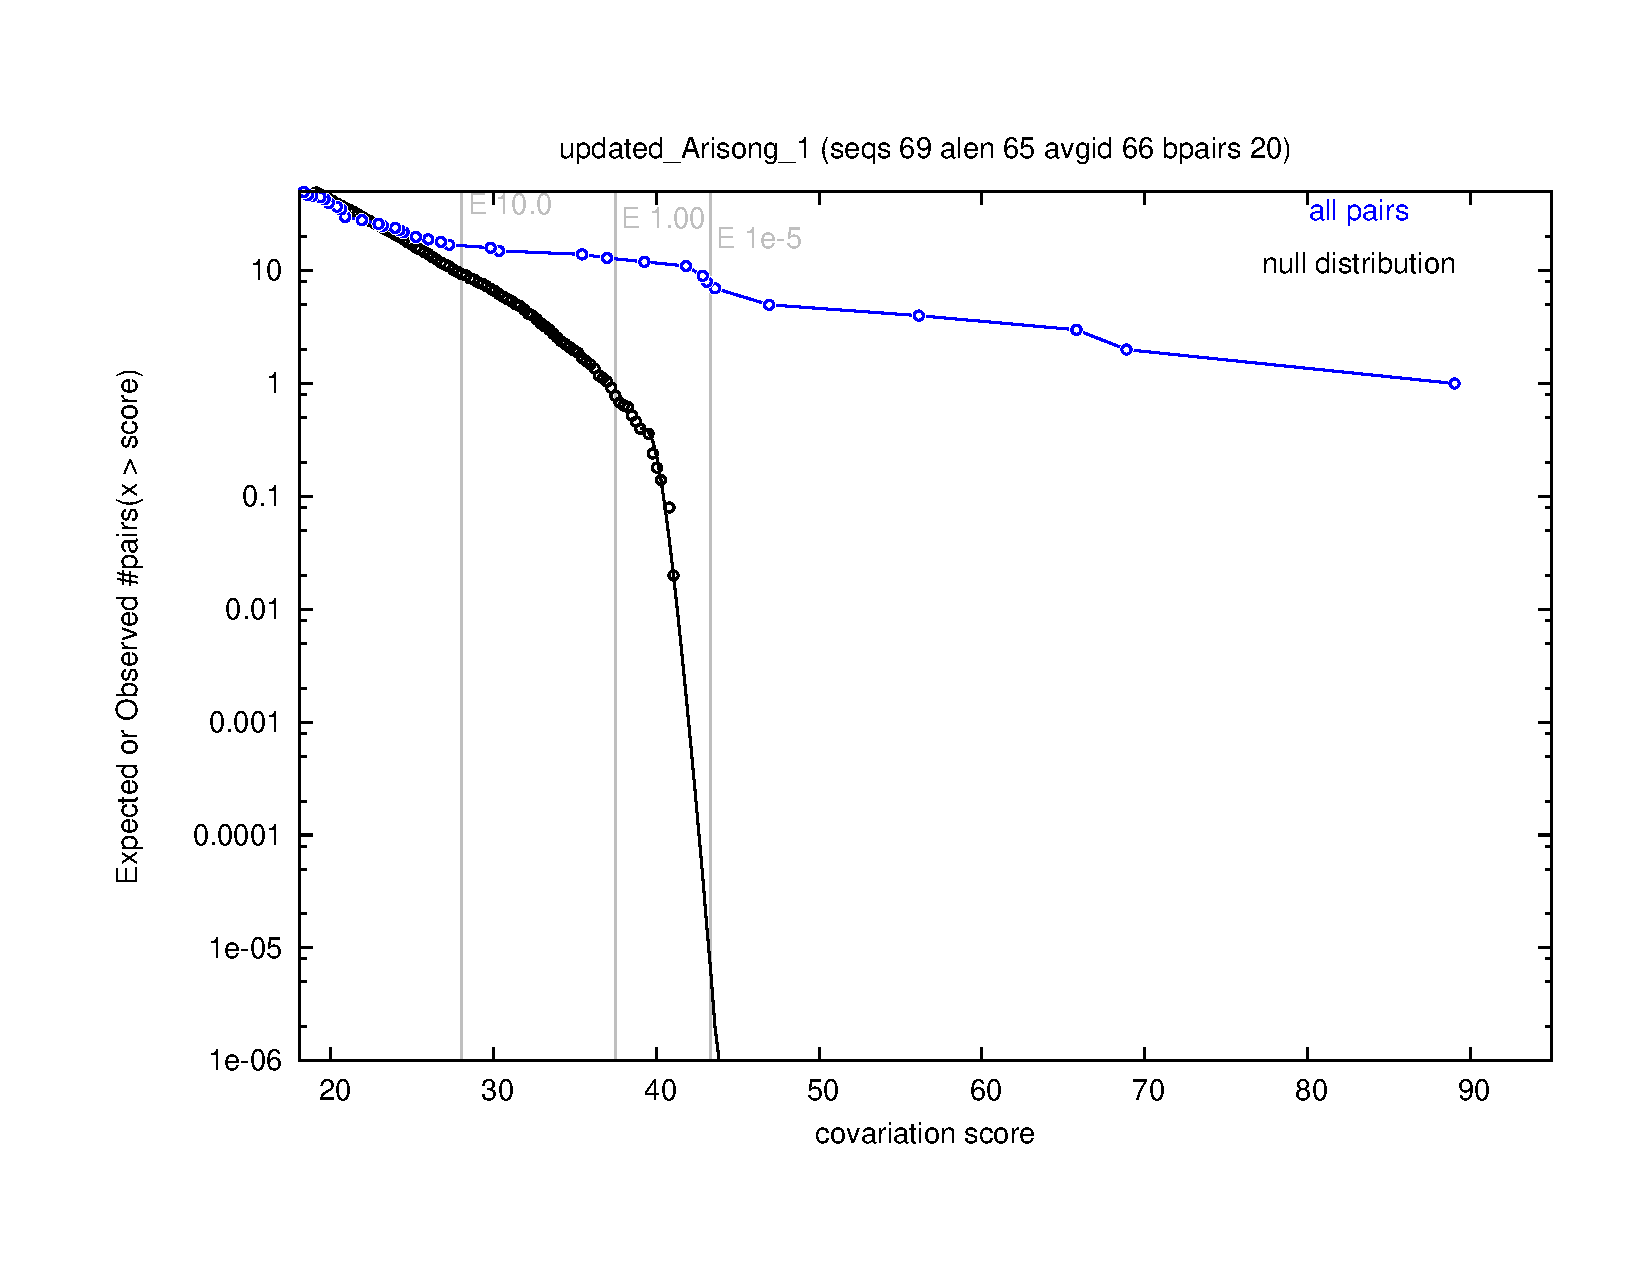
\includegraphics[scale=0.50]{Arisong_his.pdf} 
 \caption{\small\textbf{\emprog{tutorial/updated\_Arisong\_1.cdf.\{ps,svg\}}:
     covariation scores cdf.}  The cdf of scores for all
   pairs in the given alignment is depicted in blue. The cdf for
   the null alignments is depicted in black. A black line indicates to
   fit to a truncated Gamma distribution of the tail of the null
   distribution. In red, we plot the cdf of scores for the pairs
   in the given alignment excluding those proposed as base pairs.}
 \label{fig:cdf}
 \end{figure}

 \begin{figure}[h] 
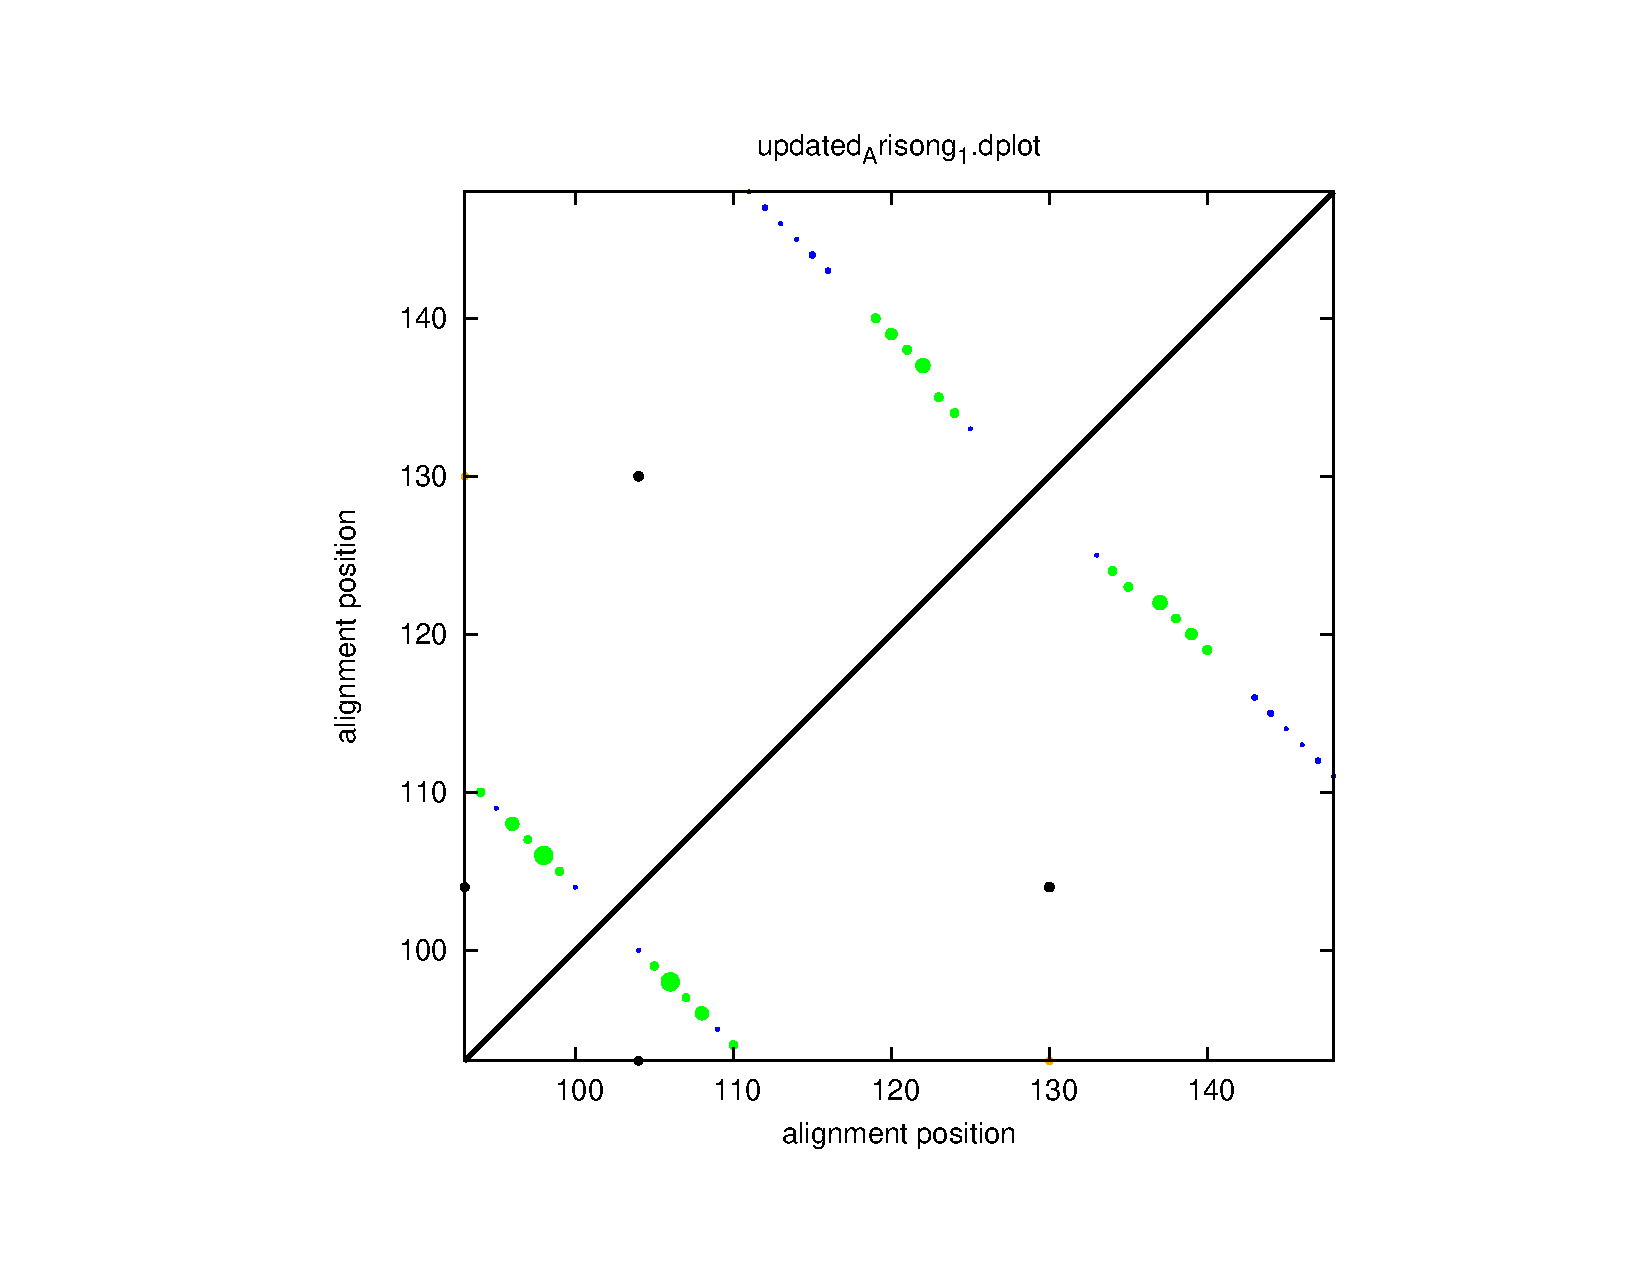
\includegraphics[scale=0.60]{Arisong_dplot.pdf} 
 \caption{\small\textbf{\emprog{tutorial/updated\_Arisong\_1.dplot.\{ps,svg\}}:
   dotplot.}  Dot size is proportional to the covariation score. In
   blue we depict the consensus base pairs; in green, the consensus
   base pairs that show significant covariation; in orange (none shown
   in this plot), we depict other pairs that have significant
   covariation, are not part of the consensus secondary structure but
   are compatible with it; in black we depict other significant pairs.
   Position are relative to the original input alignment (before any
   gapped column is removed).}
\label{fig:dplot} 
\end{figure}



 

